\documentclass[aspectratio=169]{beamer}
\usepackage[utf8]{inputenc}
\usepackage{ulem}
\usepackage{xcolor}
\usepackage{listings}
\usepackage{tikz}
\usepackage{multimedia}
\lstset{
  backgroundcolor=\color{white},   % choose the background color; you must add \usepackage{color} or \usepackage{xcolor}; should come as last argument
  basicstyle=\footnotesize\ttfamily,        % the size of the fonts that are used for the code
  breakatwhitespace=false,         % sets if automatic breaks should only happen at whitespace
  breaklines=true,                 % sets automatic line breaking
  captionpos=b,                    % sets the caption-position to bottom
  commentstyle=\color{gray},    % comment style
  deletekeywords={...},            % if you want to delete keywords from the given language
  escapeinside={\%*}{*)},          % if you want to add LaTeX within your code
  extendedchars=true,              % lets you use non-ASCII characters; for 8-bits encodings only, does not work with UTF-8
  frame=single,                    % adds a frame around the code
  keepspaces=true,                 % keeps spaces in text, useful for keeping indentation of code (possibly needs columns=flexible)
  keywordstyle=\color{blue},       % keyword style
  language=bash,                 % the language of the code
  morekeywords={*,...},            % if you want to add more keywords to the set
  numbers=left,                    % where to put the line-numbers; possible values are (none, left, right)
  numbersep=5pt,                   % how far the line-numbers are from the code
  numberstyle=\tiny\color{gray},   % the style that is used for the line-numbers
  rulecolor=\color{black},         % if not set, the frame-color may be changed on line-breaks within not-black text (e.g. comments (green here))
  showspaces=false,                % show spaces everywhere adding particular underscores; it overrides 'showstringspaces'
  showstringspaces=false,          % underline spaces within strings only
  showtabs=false,                  % show tabs within strings adding particular underscores
  stepnumber=1,                    % the step between two line-numbers. If it's 1, each line will be numbered
  stringstyle=\color{teal},        % string literal style
  tabsize=2,                       % sets default tabsize to 2 spaces
  title=\lstname,                  % show the filename of files included with \lstinputlisting; also try caption instead of title
  columns=fullflexible,            % Less spacing between characters
  literate={á}{{\'a}}1 {ã}{{\~a}}1 {é}{{\'e}}1,
}
\lstdefinestyle{base}{
  langage=bash,
  moredelim=**[is][\color{red}]{@}{@},
}

\usetheme{Rochester}
\beamersetuncovermixins{\opaqueness<1>{25}}{\opaqueness<2->{15}}
\newcommand{\light}[1]{\sout{\textcolor{gray}{#1}}}
\newcommand{\shell}[1]{\textcolor{brown}{#1}}
\newcommand{\cont}[1]{\textcolor{orange}{#1}}
\newcommand{\err}[1]{\textcolor{red}{#1}}

%\definecolor{orange_smile}{RGB}{225, 128, 84}
%\setbeamercolor*{frametitle}{parent=orange_smile}

\definecolor{UBCblue}{rgb}{0.04706, 0.13725, 0.26667} % UBC Blue (primary)
%\definecolor{OrangeSMILE}{rgb}{0.88235, 0.50196, 0.32941} % UBC Blue (primary)

\usecolortheme[named=UBCblue]{structure}



\AtBeginSection[] % Do nothing for \section*
{
\begin{frame}
  \frametitle{Outline}
  \tableofcontents[currentsection]
\end{frame}
}

%\setbeamertemplate{navigation symbols}{}

% #############################################################################
%   BEGIN DOCUMENT
% #############################################################################

\title{THE MOUSE IS LAVA \\ Change your habits, boost your productivity}
\author[shortname]{Rayan Mac\\[2mm]\footnotesize{with special thanks to Kamel Hacene\\for his valuable advice}}
\date{2019-10-09}
\titlegraphic{
\includegraphics[scale=0.02]{./images/logoCC_minimalist}}
\begin{document}

% =============================================================================
%   Title / Table of contents


\begin{frame}
  \titlepage
\end{frame}

\section*{Context}

\begin{frame}
  \frametitle{This is Bob}
    \begin{figure}[h]
        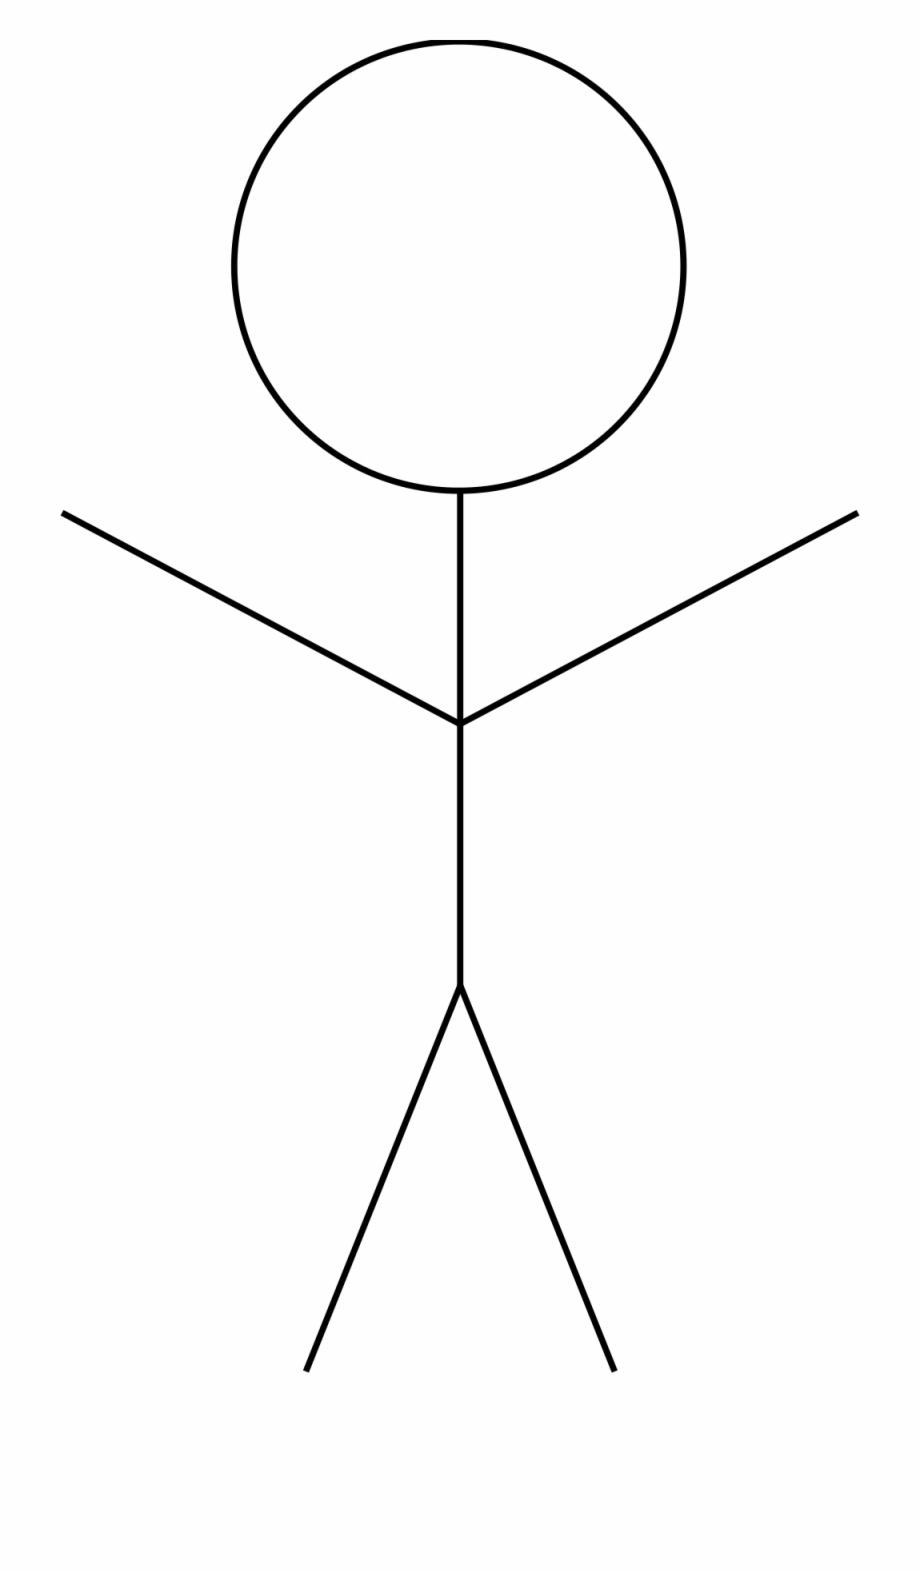
\includegraphics[scale=0.10]{./images/stickman.png}
    \end{figure}
\end{frame}


\begin{frame}
  \frametitle{Why reduce use of the mouse ?}
  \begin{itemize}
    \item Gain in efficiency
    \item Best window management
        \pause
    \item Mouse is not working / too far
  \end{itemize}
\end{frame}

\begin{frame}
  \frametitle{Goal : Complete everyday tasks only using keyboard}
  \begin{itemize}
    \item Open and close apps quickly
    \item Switch between windows easily
    \item Share resources between windows
    \item Navigate the web
  \end{itemize}
\end{frame}

% =============================================================================
%   PART 1
%

\begin{frame}[c]
    %\frametitle{A first slide}
    \begin{center}
        \huge PART 1 : Adapt your environment
    \end{center}
\end{frame}

\section{Shortcuts everywhere}
\subsection{Default and alternatives}

\begin{frame}
 \frametitle{Starting point}
    \begin{figure}[h]
        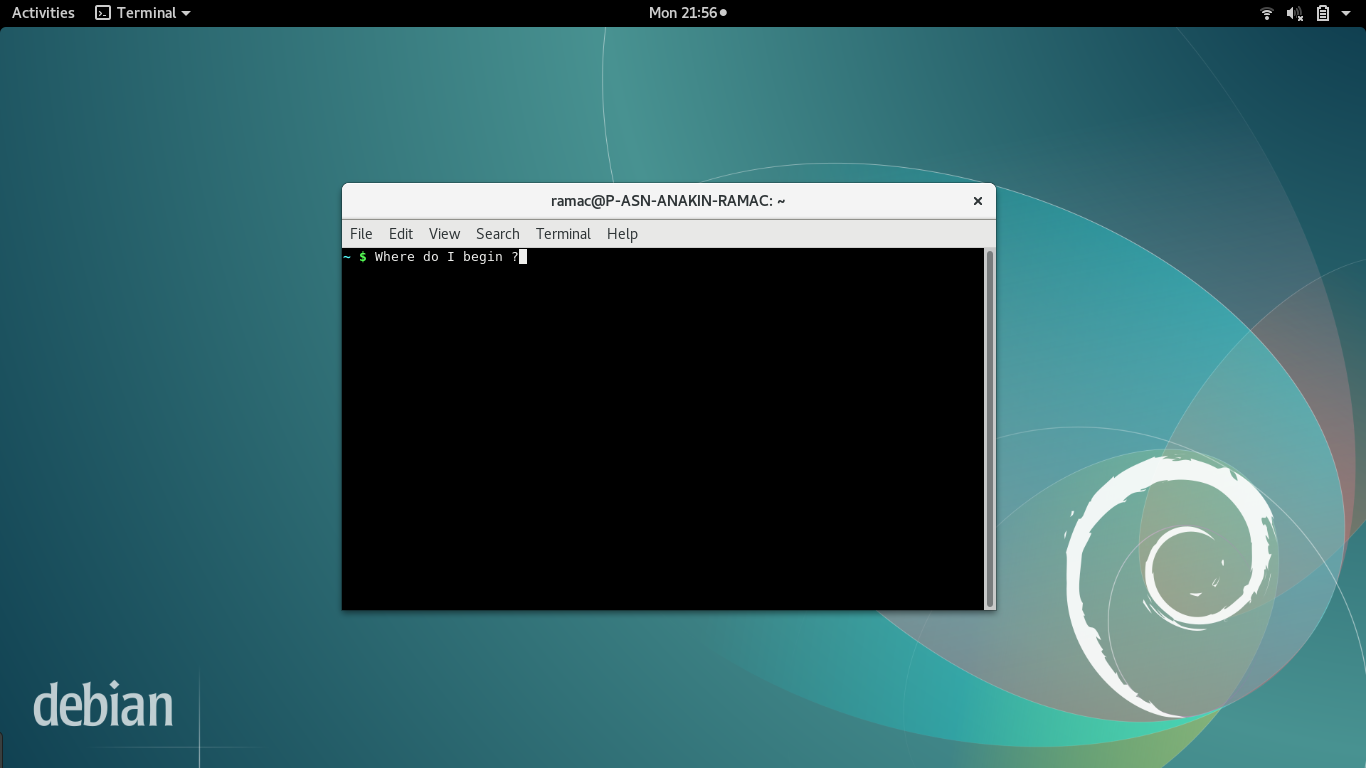
\includegraphics[scale=0.23]{./images/starting_point.png}
    \end{figure}
\end{frame}

\begin{frame}[fragile]
    \frametitle{Shortcuts management}
  \begin{itemize}
    \item Default shortcuts
    \item xbindkeys : ~/.xbindkeysrc
    \item sxhkd : ~/.sxhkdrc
  \end{itemize}
  \begin{lstlisting}
    # terminal emulator
    super + Return
        urxvt
    # focus the node for the given path jump
    super + \{p,b,comma,period\}
        bspc node -f \@\{parent,brother,first,second\}
   \end{lstlisting}
\end{frame}

\section{Terminal multiplexers}
\subsection{Architecture}
\subsection{Features}
\subsection{Practical use}

\begin{frame}
  \frametitle{Definition}
  A terminal multiplexer allows multiple sessions and applications to be displayed and managed on a single screen.
    \begin{figure}[h]
        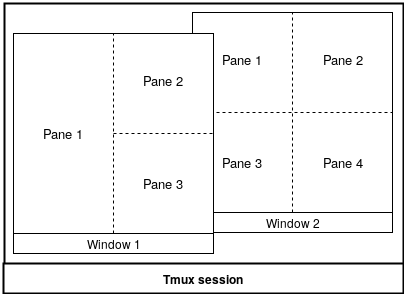
\includegraphics[scale=0.5]{./images/tmux_panes.png}
    \end{figure}
\end{frame}

\begin{frame}
  \frametitle{Architecture}
    \begin{figure}[h]
        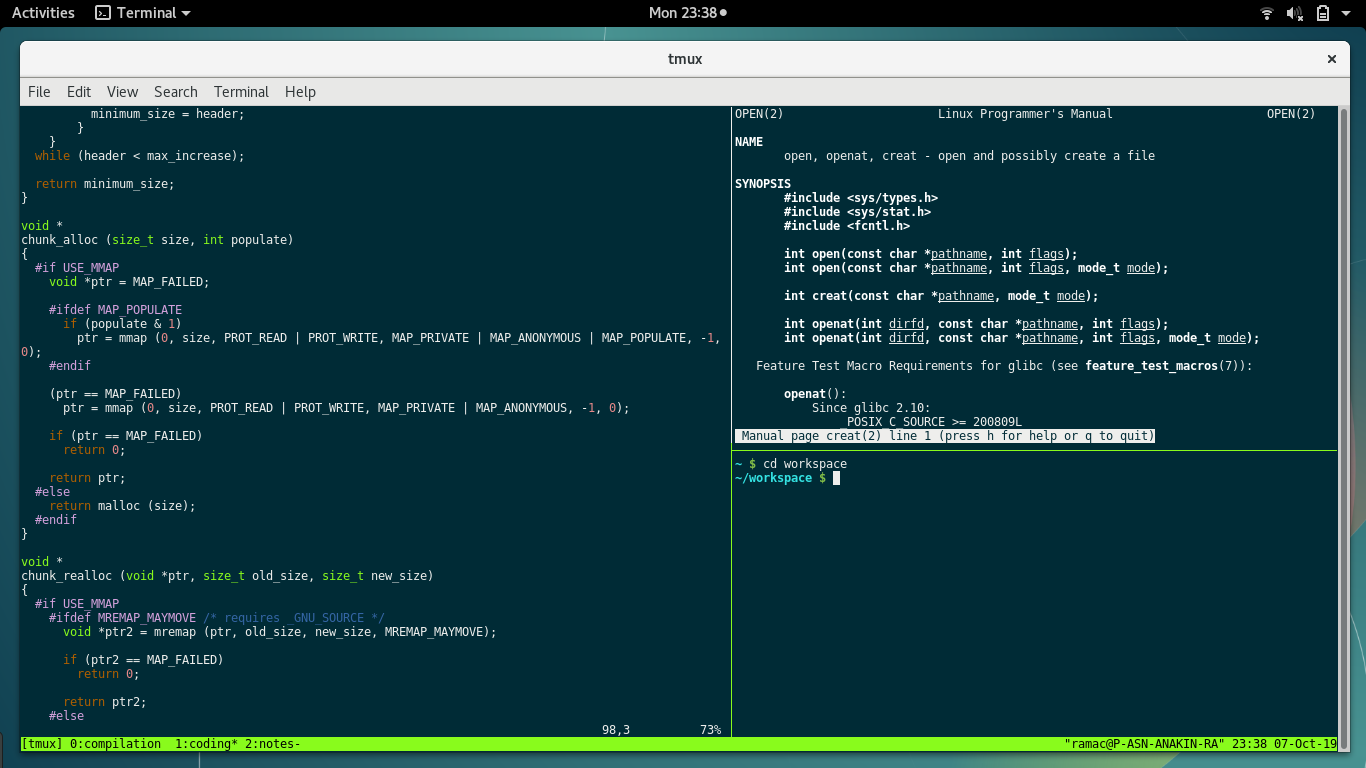
\includegraphics[scale=0.23]{./images/tmux_visual.png}
    \end{figure}
\end{frame}

\begin{frame}
  \frametitle{Popular Terminal multiplexers}
    Historically, GNU Screen 1987 \newline

    Nowadays:
    \begin{itemize}
      \item Terminator
      \item Screen
      \item Tmux
      \item Byobu
    \end{itemize}
\end{frame}

\begin{frame}
  \frametitle{Practical use}
    \begin{center}
      \movie[height=6.5cm, width=11.55cm]{PLAY VIDEO}{../videos/tmux.mp4}
    \end{center}
\end{frame}


\section{Go Tiling !}
\subsection{WMs and TWMs}
\subsection{Installation and configuration}
\subsection{Practical use}

\begin{frame}
    \frametitle{About windows manager}
  Window manager: A system software controlling the placement and appareance of windows inside a graphical user interface.\newline
    \begin{figure}[h]
        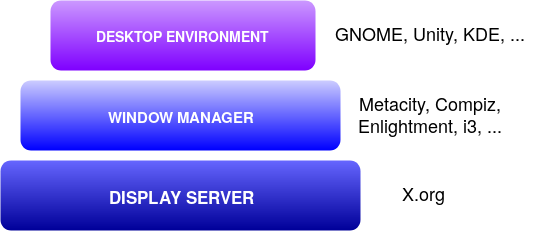
\includegraphics[scale=0.5]{./images/windows_stack.png}
    \end{figure}
\end{frame}

\begin{frame}
    \frametitle{Tiling window managers}
    Organize windows automatically so that they don’t overlap, while maximizing the space use.\newline

    Benefits:
    \begin{itemize}
      \item Keep at sight the whole working environment
      \item Lighter and faster than usual WMs
      \item Built-in shortcuts optimized for keyboards
    \end{itemize}
\end{frame}

\begin{frame}
    \frametitle{Struggling with windows arrangement: DAY 1}
    \begin{figure}[h]
        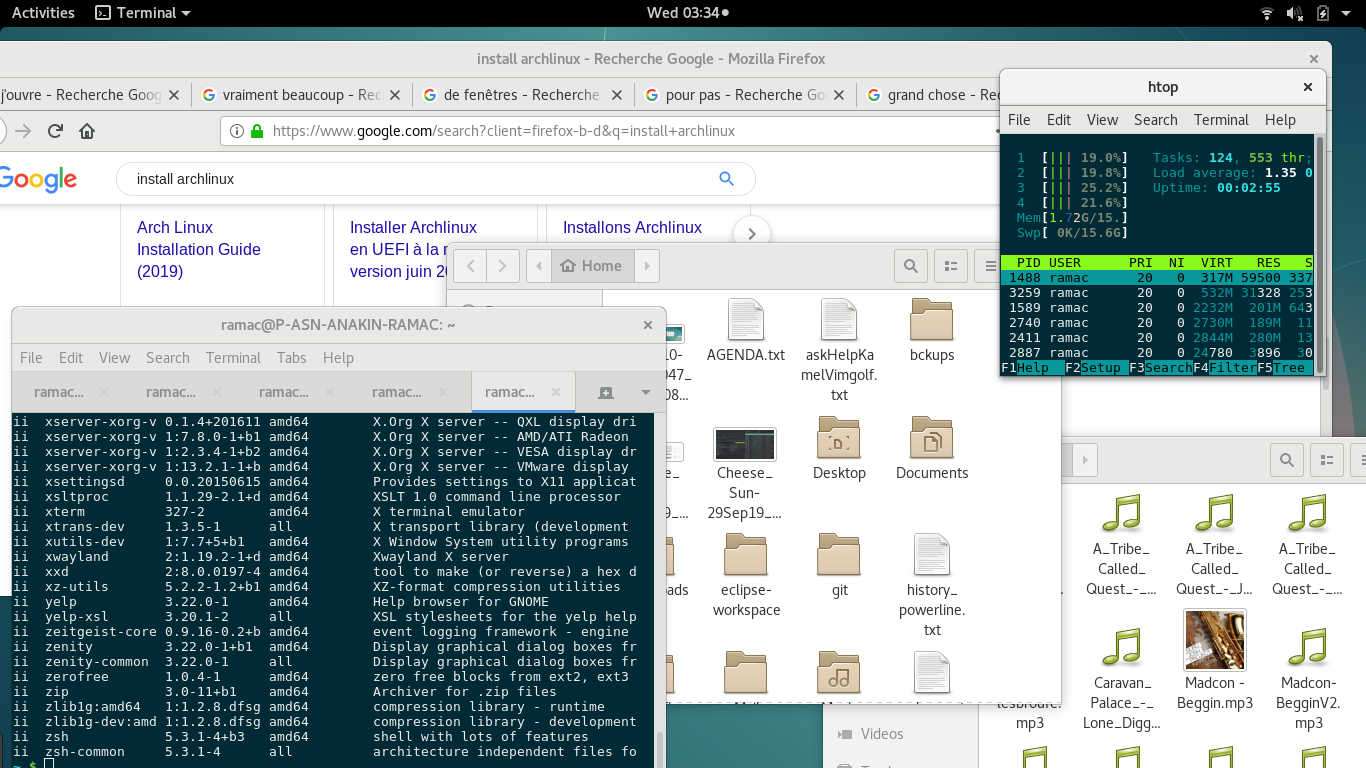
\includegraphics[scale=0.23]{./images/messy_wp.png}
    \end{figure}
\end{frame}

\begin{frame}
    \frametitle{Struggling with windows arrangement: DAY 2}
    \begin{figure}[h]
        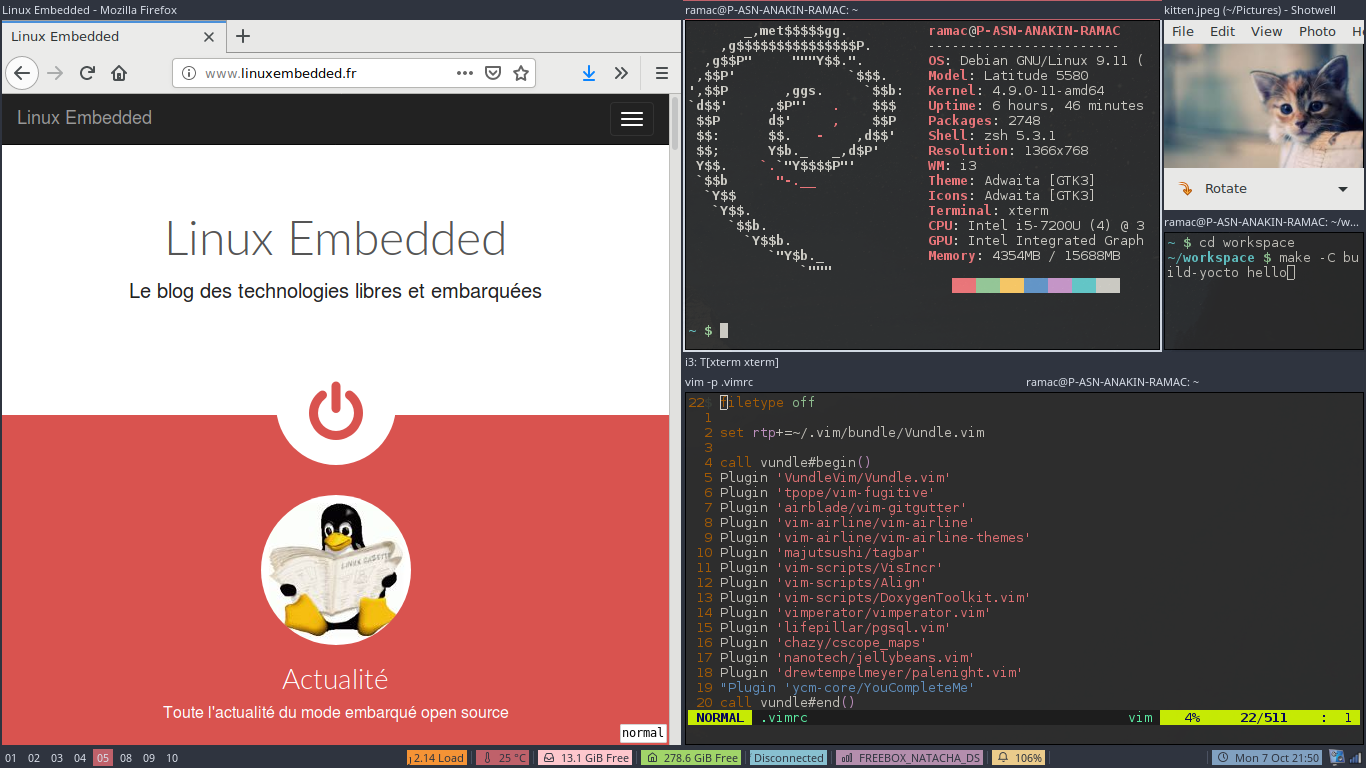
\includegraphics[scale=0.23]{./images/organized_wp.png}
    \end{figure}
\end{frame}

\begin{frame}
    \frametitle{Popular TWMs}
    \begin{itemize}
      \item i3 / sway : user friendly, huge community and great documentation
      \item Awesome (lua) : great mouse integration, highly configurable
      \item dwm (C), xmonad (haskell) : small, fast, simple
      \item bspwm : very light, high degree of customisation
      \item [...]
    \end{itemize}
\end{frame}

\begin{frame}
    \frametitle{Installation}
    Usually available in official repositories
    \begin{figure}[h]
        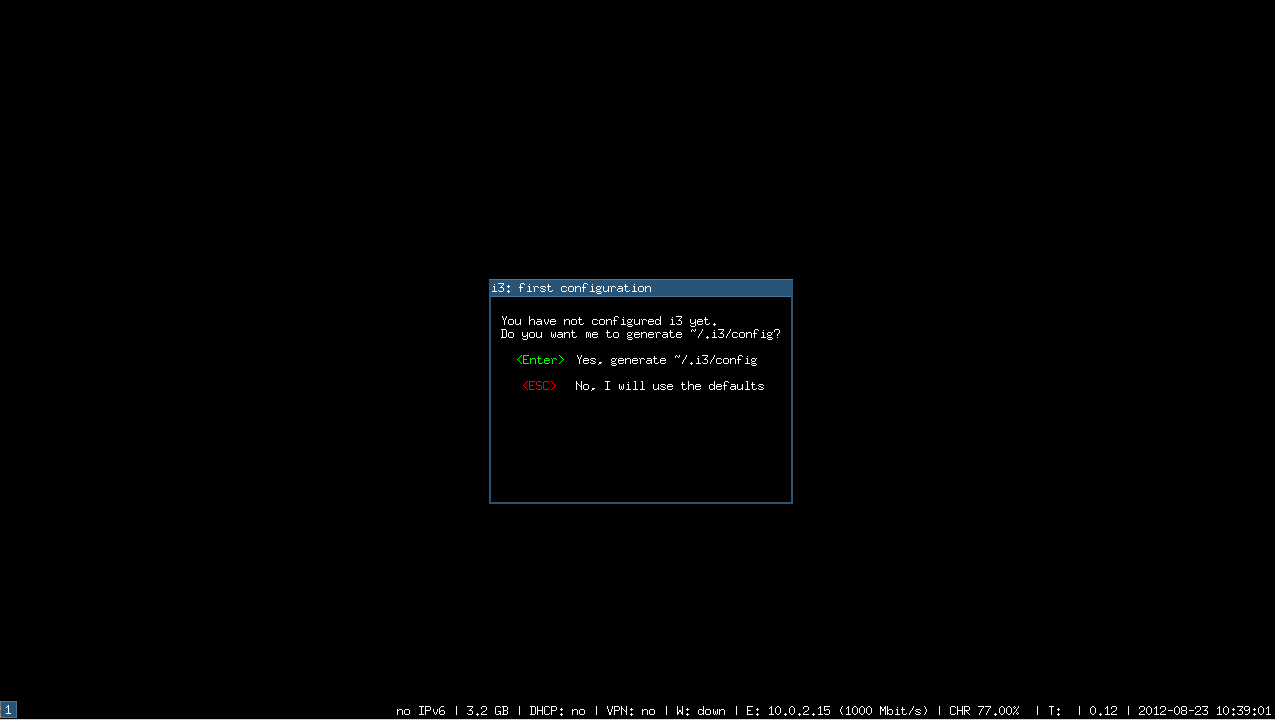
\includegraphics[scale=0.23]{./images/i3starting.png}
    \end{figure}
\end{frame}

\begin{frame}[fragile]
    \frametitle{Configuration (i3 example)}
    A single configuration file :  ~/.config/i3/config
    \begin{lstlisting}
    # enter fullscreen mode for the focused container
    bindsym $mod+f fullscreen toggle

    # colour of border, background, text, indicator, and child_border
    client.focused              #bf616a #2f343f #d8dee8 #bf616a #d8dee8

    # add network-manager status bar shortcut
    exec --no-startup-id nm-applet
    \end{lstlisting}

    Make it look eye-candy : i3-starterpack \newline

    git clone https://github.com/ramacassis/confighamac.git
\end{frame}

\begin{frame}
  \frametitle{Practical use}
    \begin{center}
      \movie[height=6.5cm, width=11.55cm]{PLAY VIDEO}{../videos/demo_i3.mp4}
    \end{center}
\end{frame}

\section{Useful tools}
\subsection{Clipboard managers}

\begin{frame}
    \frametitle{Linux clipboard}
    \begin{figure}[h]
        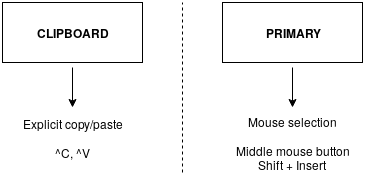
\includegraphics[scale=0.6]{./images/linux_clipboard.png}
    \end{figure}
    \begin{itemize}
    \item Access clipboard in command line: xclip
   % \item \verb|[pwdc='pwd \| tr -d "\n" \| xclip']|
   % \item Add time-saving aliases: pwdc='pwd | tr -d "\n" | xclip'\newline
    \item Other clipboard manager: clipit, copyq, […]
    \end{itemize}
\end{frame}

%PART 2

\begin{frame}[c]
    \begin{center}
        \huge PART 2: Expand to other apps !
    \end{center}
\end{frame}

\begin{frame}
    \frametitle{Web navigation}
    General idea: use (vim) shortcuts as an interface to browser\newline

    Historically:
    \begin{itemize}
    \item Vimperator
    \item Pentadactyl\newline
    \end{itemize}

    Nowadays:
    \begin{itemize}
    \item Tridactyl
    \item Vim-vixen
    \item cVim
    \item [...]
    \end{itemize}
\end{frame}

\begin{frame}
    \frametitle{All tools put together}
    \begin{center}
      \movie[height=6.5cm, width=11.55cm]{PLAY VIDEO}{../videos/global.mp4}
    \end{center}
\end{frame}

\begin{frame}
    \frametitle{Conclusion}
    \begin{itemize}
    \item Open and close apps quickly: shortcuts, TWM
    \item Switch between windows easily: terminal multiplexers, TWM
    \item Share resources between windows: clipboard, command history
    \item Navigate the web : browser plugins, CLI apps
    \end{itemize}
\end{frame}

\begin{frame}
    \frametitle{What's next ?}
    Going further...\newline
    \begin{itemize}
    \item Web: elinks, lynx
    \item Mail: mutt, neomutt, alpine
    \item Calendar: calcurse, remind
    \item Music: mpsyt, cmus\newline
    \end{itemize}

    https://wiki.archlinux.org/index.php/list\_of\_applications
    https://doc.ubuntu-fr.org/liste\_des\_applications\_console\newline

    Find the compromise that suits your needs !
\end{frame}

\begin{frame}[c]
    \begin{center}
        \Huge Thanks for your attention \\ \huge Let's share !
    \end{center}
\end{frame}

\end{document}
